%% start of file `template.tex'.
%% Copyright 2006-2015 Xavier Danaux (xdanaux@gmail.com).
%
% Adapted to be an Rmarkdown template by Mitchell O'Hara-Wild
% 8 February 2019
%
% This work may be distributed and/or modified under the
% conditions of the LaTeX Project Public License version 1.3c,
% available at http://www.latex-project.org/lppl/.


\documentclass[11pt,a4paper,]{moderncv}

% moderncv themes
\moderncvstyle{casual}                             % style options are 'casual' (default), 'classic', 'banking', 'oldstyle' and 'fancy'

\definecolor{color0}{rgb}{0,0,0}% black
\definecolor{color1}{HTML}{414141}% custom
\definecolor{color2}{rgb}{0.45,0.45,0.45}% dark grey

\usepackage[scaled=0.86]{DejaVuSansMono}

\providecommand{\tightlist}{%
	\setlength{\itemsep}{0pt}\setlength{\parskip}{0pt}}
\def\donothing#1{#1}
\def\emaillink#1{#1}

%\nopagenumbers{}                                  % uncomment to suppress automatic page numbering for CVs longer than one page

% character encoding
%\usepackage[utf8]{inputenc}                       % if you are not using xelatex ou lualatex, replace by the encoding you are using
%\usepackage{CJKutf8}                              % if you need to use CJK to typeset your resume in Chinese, Japanese or Korean

% adjust the page margins
\usepackage[scale=0.75,footskip=60pt]{geometry}
%\setlength{\hintscolumnwidth}{3cm}                % if you want to change the width of the column with the dates
%\setlength{\makecvheadnamewidth}{10cm}            % for the 'classic' style, if you want to force the width allocated to your name and avoid line breaks. be careful though, the length is normally calculated to avoid any overlap with your personal info; use this at your own typographical risks...


\usepackage{fancyhdr}
\pagestyle{fancy}
\fancyhf{}
\fancyhead[R]{\thepage}

% personal data
\name{Sarah E}{Schwartz}
\title{Research Assistant Professor}
\address{Utah State University}{}{}
\phone[mobile]{(435) 797 - 0169} % Phone number
\email{\donothing{\href{mailto:Sarah.Schwartz@usu.edu}{\nolinkurl{Sarah.Schwartz@usu.edu}}}}
\homepage{www.SarahSchwartzStats.com} % Personal website
\social[linkedin]{SarBearSchwartz}
\social[twitter]{USU\_StatStudio}
\social[github]{SarBearSchwartz}
% \extrainfo{additional information}                 % optional, remove / comment the line if not wanted



\quote{I am a statistician with a passion for facilitating research that
is appropriate, transparent, and reproducible.}

% Pandoc CSL macros
\newlength{\cslhangindent}
\setlength{\cslhangindent}{1.5em}
\newlength{\csllabelwidth}
\setlength{\csllabelwidth}{3em}
\newenvironment{CSLReferences}[3] % #1 hanging-ident, #2 entry spacing
 {% don't indent paragraphs
  \setlength{\parindent}{0pt}
  % turn on hanging indent if param 1 is 1
  \ifodd #1 \everypar{\setlength{\hangindent}{\cslhangindent}}\ignorespaces\fi
  % set entry spacing
  \ifnum #2 > 0
  \setlength{\parskip}{#2\baselineskip}
  \fi
 }%
 {}
\usepackage{calc}
\newcommand{\CSLBlock}[1]{#1\hfill\break}
\newcommand{\CSLLeftMargin}[1]{\parbox[t]{\csllabelwidth}{#1}}
\newcommand{\CSLRightInline}[1]{\parbox[t]{\linewidth - \csllabelwidth}{#1}}
\newcommand{\CSLIndent}[1]{\hspace{\cslhangindent}#1}

%----------------------------------------------------------------------------------
%            content
%----------------------------------------------------------------------------------
\begin{document}
%\begin{CJK*}{UTF8}{gbsn}                          % to typeset your resume in Chinese using CJK
%-----       resume       ---------------------------------------------------------
\makecvtitle



\hypertarget{academic-appointment}{%
\section{Academic Appointment}\label{academic-appointment}}

\nopagebreak
    \cventry{2015-present}{Assistant Research Professor}{Psychology Department, College of Education and Human Services}{Utah State University}{}{\begin{itemize}%
\item Director, The Statistical Consulting Studio%
\item Instructor, graduate student quantitatice methods and statistics courses%
\end{itemize}}
    \cventry{2013-2015}{Statistician}{Office of Research Services, College of Education and Human Services}{Utah State University}{}{\begin{itemize}%
\item Acting Director, Office of Methodological and Data Sciences%
\item Instructor, graduate student quantitatice methods and statistics courses%
\end{itemize}}
    \cventry{2005-2013}{Statistician and Data Manager}{Center for Epidemiology}{Utah State University}{}{\begin{itemize}%
\item Managed databases, clean data, and prepare custom datasets%
\item Performed statistical analyses and prepared publications, posters, presentations,
and grant submissions%
\item Worked under three main grants and many co-investigators: University of Utah,
  BYU, Duke, John Hopkins, University of Maryland, ect.%
\end{itemize}}
    \cventry{2012}{Data Manager}{Kenoi Genetics Lab}{Brigham Young University}{}{\begin{itemize}%
\item Managed databases and prepare custom datasets%
\end{itemize}}
    \cventry{2006-2008}{Adjunct Lecturer}{Mathematics and Statistics Department}{Utah State University}{}{\begin{itemize}%
\item Traditional, evening, and distance courses%
\end{itemize}}
    \cventry{2000-2004}{High School Teacher, Math and Science}{Mathematics and Statistics Department}{Utah State University}{}{\begin{itemize}%
\item Sky View High School, Smithfield, Utah%
\item Logan River Academy, Logan, Utah%
\end{itemize}}

\vspace{5 mm}

\hypertarget{certificates}{%
\section{Certificates}\label{certificates}}

\nopagebreak
    \cventry{2001-2009}{Teaching License}{Secondary Education}{State of Utah}{}{\begin{itemize}%
\item Endorsements: mathematics level 4 and chemistry%
\end{itemize}}

\clearpage

\hypertarget{education}{%
\section{Education}\label{education}}

\nopagebreak
    \cventry{2013-2017}{PhD: Mathetatics, Specialization in Statistics}{Utah State University}{Logan, Utah, USA}{}{\begin{itemize}%
\item TA: Lecturer and grader%
\item RA: Simulation programmer, Cytel Software Inc.%
\end{itemize}}
    \cventry{2004-2006}{MS: Statistics}{Utah State University}{Logan, Utah, USA}{}{\begin{itemize}%
\item Mentor: Dr. Chris Corcoran%
\item TA: Lecturer and grader%
\item RA: Statistician, Center for Epidemiology Studies%
\end{itemize}}
    \cventry{1998-2000}{BS: Math and Chem Secondary Education}{Utah State University}{Logan, Utah, USA}{}{\begin{itemize}%
\item Student Teaching: Sky View High School, Smithfield, Utah%
\end{itemize}}

\vspace{5 mm}

\hypertarget{awards-and-honors}{%
\section{Awards and Honors}\label{awards-and-honors}}

\nopagebreak
    \cventry{2015}{Department Academic Excellence Award}{Mathematics and Statistics Department}{Utah State University}{}{\empty}
    \cventry{2014}{Department Industrious Graduate Student Award}{Mathematics and Statistics Department}{Utah State University}{}{\empty}
    \cventry{2005}{Department Graduate Student Teacher of the Year Award}{Mathematics and Statistics Department}{Utah State University}{}{\empty}

\vspace{5 mm}

\hypertarget{software}{%
\section{Software}\label{software}}

\hypertarget{program-proficiencies}{%
\subsection{\texorpdfstring{\textbf{Program
Proficiencies}}{Program Proficiencies}}\label{program-proficiencies}}

\nopagebreak
    \cventry{}{R, R Studio, and R Markdown (LaTeX)}{}{}{}{\begin{itemize}%
\item Data cleaning and wrangling, statistical analysis, and reproducible reporting%
\end{itemize}}
    \cventry{}{SAS, SPSS, MPlus, and G*Power}{}{}{}{\begin{itemize}%
\item Data cleaning and wrangling, and statistical analysis%
\end{itemize}}
    \cventry{}{REDCap and Qualtrics}{}{}{}{\begin{itemize}%
\item Creating forms and collecting data%
\end{itemize}}

\hypertarget{open-source-project-on-github}{%
\subsection{\texorpdfstring{\textbf{Open-Source Project on
GitHub}}{Open-Source Project on GitHub}}\label{open-source-project-on-github}}

\hypertarget{refs_github_projects}{}
\leavevmode\vadjust pre{\hypertarget{ref-R-texreghelpr}{}}%
\CSLLeftMargin{1. }
\CSLRightInline{Schwartz, S. E. (2021). \emph{Texreghelpr: Extract
generalized regression output for use in `texreg` tables}.
\url{https://github.com/sarbearschwartz/texreghelpr}}

\leavevmode\vadjust pre{\hypertarget{ref-R-dissertateUSU}{}}%
\CSLLeftMargin{2. }
\CSLRightInline{Barrett, T. S., \& Schwartz, S. E. (2021).
\emph{dissertateUSU: Materials for writing a dissertation at utah state
university in r markdown}.
\url{https://github.com/TysonStanley/dissertateUSU}}

\clearpage

\hypertarget{continuing-education}{%
\section{Continuing Education}\label{continuing-education}}

\nopagebreak
    \cventry{Summer 2016}{Structural Equation Modeling in Longitudinal Research}{APA Advanced Training Institutes (ATIs)}{Arizonal State University}{}{\begin{itemize}%
\item This ATI is designed to highlight recent methodological advances in the analysis of longitudinal psychological data using structural equation modeling (SEM).%
\item The workshop covers a range of topics, including growth models, factorial invariance, incomplete data, ordinal outcomes, and latent change score models.%
\item Instructors: Dr. Craig Enders , Department of Psychology at The University of California, Los Angeles, Dr. Kevin J. Grimm of the Department of Psychology at Arizona State University, and Dr. Nilam Ram of the Departments of Psychology and Communications at Stanford University.%
\end{itemize}}
    \cventry{Fall Semester 2019}{PSY 7810: Structural Equation Modeling}{Audit granduate course}{Utah State University}{}{\begin{itemize}%
\item Objective 1) understanding the motivation, logic, and inner workings of SEM%
\item Objective 2) be able to specify models and fit them to data using conventional statistical software%
\item Objective 3)  have the ability to interpret and report results in a manner consistent with the standards of peer-reviewed journals%
\item Instructor: Dr. Sarfraz Serang%
\end{itemize}}
    \cventry{August 17, 2021}{The Probability Problem: Building Probability Skills in Intro Statistics}{Workshop/Seminar}{Hawkes Learning}{}{\begin{itemize}%
\item Focus: struggles that undergraduate students (non-STEM majors) tend to face with probability in their introductory statistics course.%
\item Instructional principle implemented:  worked-out problems including writing prompts to encourage self-explanation of students’ thinking through studying the worked-out examples%
\item Instructor: KimberLeigh Hadfield, Senior Lecturer USU Math and Statistics Department%
\end{itemize}}
    \cventry{October 26, 2021}{A New Normal in Inclusive, Usable Online Learning Experiences}{Workshop/Seminar}{Utah State University}{}{\begin{itemize}%
\item Office of Empowering Teaching Excellence (ETE)%
\item Thurston, T. N., Lundstrom, K., González, C., Stommel, J., Masland, L. C., Buyserie, B., ... \& Eason, A. (2021). Resilient Pedagogy: Practical Teaching Strategies to Overcome Distance, Disruption, and Distraction.%
\item Presenters/authors: Christopher Phillips and Jared Colton%
\end{itemize}}

\vspace{7mm}

\hypertarget{administrative}{%
\section{Administrative}\label{administrative}}

\nopagebreak
    \cventry{2018-present}{CEHS Office of Research}{EDUC 6600 Pre-Test Coordinator}{Utah State University}{}{\begin{itemize}%
\item Update pre-test question bank%
\item Moderate Student communication and answer questions.%
\item Setup remote test taking with advent of Covid-19 shift to online.%
\item Create and monitor refresher materials for test-prep%
\item Monitor suspisous behavior and check for cheating%
\item Interface with all CEHS departments on the expectations and timeline.%
\end{itemize}}

\clearpage

\hypertarget{teaching-experience-graduate-level}{%
\section{Teaching Experience: Graduate
Level}\label{teaching-experience-graduate-level}}

\nopagebreak
    \cventry{Fall: 2016-present}{Psychology Department}{PSY 7650: Multilevel and Marginal Models}{Utah State University}{}{\begin{itemize}%
\item Coverage of multilevel (ie, mixed-effects, hierarchical linear) and marginal (ie, GEE) models for both continuous and categorical outcomes.%
\item Includes application of these methods to many types of cross-sectional and longitudinal research designs (eg, experimental, case-control, cohort, cross-over, complex sample, randomized controlled trials).%
\item Software: R and R Studio%
\item Online eBook: all class examples with code and explainations%
\item Youtube: Pre-recorded lectures for course when Covid-19 induced a shift to online, asynchronous learing%
\end{itemize}}
    \cventry{Spring/Sum 2015-present}{CEHS: Office of Research Services}{EDUC 6600:  Statistical Foundataions (previously: Research Design and Analysis I)}{Utah State University}{}{\begin{itemize}%
\item Research design and statistical concepts for research in education, human services, and psychology, with emphasis on the selection and interpretation of statistical analyses.%
\item Focus on inference and ANOVA based methods. Includes a combination of traditional face-to-face and distance-site students.%
\item Software: R and R Studio starting in 2018, SPSS prior%
\item Online eBook: all class examples with code and explainations%
\item Assignments online through Atomic Assessment within Canvas%
\item Youtube: Pre-recorded lectures for course when Covid-19 induced a shift to online, asynchronous learing%
\end{itemize}}

\vspace{7 mm}

\hypertarget{teaching-experience-undergraduate-level}{%
\section{Teaching Experience: Undergraduate
Level}\label{teaching-experience-undergraduate-level}}

\nopagebreak
    \cventry{Spring 2022}{Psychology Department}{PSY 3010: Psycological Statistics}{Utah State University}{}{\begin{itemize}%
\item Descriptive and inferential statistical methods.%
\item Focus on behavior statistics and statistical applications.%
\end{itemize}}
    \cventry{Spring/Fall: 2005, 2014}{Mathematics and Statistics Department}{STAT 2000: Statistical Methods}{Utah State University}{}{\begin{itemize}%
\item Introduction to statistical concepts, graphical techniques, probability, distributions, estimation, one and two sample testing, chi-square tests, and simple linear regression, one-way ANOVA.%
\item Software: StatCrunch%
\end{itemize}}
    \cventry{2008 Spring, 2007 Spring/Fall, 2006 Fall}{Mathematics and Statistics Department}{STAT 1040: Introduction to Statistics}{Utah State University}{}{\begin{itemize}%
\item Descriptive and inferential statistical methods.%
\item Emphasis on conceptual understanding and statistical thinking.%
\item Examples presented from many different areas.%
\item Software: none%
\end{itemize}}
    \cventry{Fall 2004}{Mathematics and Statistics Department}{MATH 1050: College Algebra}{Utah State University}{}{\begin{itemize}%
\item Functions: graphs, transformations, combinations, and inverses.%
\item Polynomial, rational, exponential, logarithmic functions, and applications.%
\item Systems of equations and matrices. Partial fractions.%
\item Software: graphing calculators%
\end{itemize}}
    \cventry{Summer 2006}{Mathematics and Statistics Department}{MATH 1010: Intermediate Algebra}{Utah State University}{}{\begin{itemize}%
\item Review of introductory algebra concepts.%
\item Topics include manipulating and simplifying expressions, solving equations and inequalities, graphing equations, and inequalities.%
\item Real world applications including linear, quadratic, polynomial, rational, exponential, and radical functions.%
\item Software: none%
\end{itemize}}

\vspace{7 mm}

\hypertarget{teaching-experience-college-wide-workshops}{%
\section{Teaching Experience: College-wide
Workshops}\label{teaching-experience-college-wide-workshops}}

\begin{quote}
\textsc{All sessions target the audience of faculty, research staff, adn graduate students in the college.  Starting in the Fall of 2019, the workshops were formalized to all enrollment for continuing education (1 CEU) or standard university credit (0.5 cr), in addition to the pervious a'la cart option.}
\end{quote}

\nopagebreak
    \cventry{Spring 2022}{Seven 1-hour sessions}{Time-to-Event Analysis, aka Survival Analysis}{Utah State University}{}{\begin{itemize}%
\item Inferior Models: You must make a choice - censoring and duration of follow-up%
\item Non-parametric approach: Kaplan Meyer Plots with Log Rank Test (bivariate)%
\item Semi-parametric approach: Cox Proportional-Hazards Regression (multivariate)%
\item Extension: Time varying covariates in a Cox model%
\end{itemize}}
    \cventry{Fall 2021}{Seven 1-hour sessions}{Categorical Data Analysis}{Utah State University}{}{\begin{itemize}%
\item Exact, permutation/bootstrap, and parametric methods%
\item GLM: Binary logistic regression%
\item GLM: Count outcomes: poisson regression, overdispersion, and negative binomial regression%
\item GLM: Zero inflated models (ZIP and ZINB)%
\end{itemize}}
    \cventry{Spring 2021}{Seven 1-hour sessions}{Missing Data and Multiple Imputations}{Utah State University}{}{\begin{itemize}%
\item Missing Data Mechanisms, Implications and Testing%
\item Historical Methos and Reporting Missing Data%
\item Multiple Imputations: basic and advanced topics%
\end{itemize}}
    \cventry{Fall 2020}{Seven 1-hour sessions}{Extensions to Regression}{Utah State University}{}{\begin{itemize}%
\item Multiple Linear Regression Refresher%
\item Powerful Publishable Plots: The Grammer of Graphics%
\item Time-to-Event Modeling: Survival Analysis%
\item Intro to Multileel and Marginal Modles: MLM, HLM, GEE%
\end{itemize}}
    \cventry{Spring 2020}{Seven 1-hour sessions}{Common Design Issues}{Utah State University}{}{\begin{itemize}%
\item Effect Size and Power Analysis uisng G*Power and R%
\item Propensity Score Matching and Alternatives%
\item Missing Data and Multiple Imputations%
\end{itemize}}
    \cventry{Fall 2019}{Seven 1-hour sessions}{Extensions to Regressio}{Utah State University}{}{\begin{itemize}%
\item Review of Regression (MLR and GLM), including creating tables and figures for publication%
\item Time-to-event/Survival Analysis: including KM plots with Log-Rank test (bivariate), Cox-PH\_Regression (multivariate)%
\item Regularized Regression (Ridge and LASSO)%
\item Intro to Multileel and Marginal Modles: MLM, HLM, GEE%
\end{itemize}}
    \cventry{2015-2020}{Two-three hour workshop}{Stand-along Sessions}{Utah State University}{}{\begin{itemize}%
\item Effect Size and Power Analysis uisng G*Power (fall 2015, fall 2017, fall 2018)%
\item Exact Methods for Categorical Data in SPSS, R, and StatXact (spring 2018)%
\item Exploring your Data with ggplot in R (spring 2016)%
\item GEE: General Estimating Equations (spring 2017)%
\item Intro to Multileel and Marginal Modles: MLM, HLM, GEE  (spring 2018, spring 2019)%
\item Intro to R and Rstudio for Absolute Beginners (fall 2015)%
\item Intro to R: The Tidyverse (fall 2016)%
\item Logistic Regression (fall 2017)%
\item Missing Data and Multiple Imputations (fall 2018)%
\item Multiple Linear Regression Refresher in SPSS and R (spring 2018)%
\item Powerful Publishable Plots: The Grammer of Graphics (spring 2016, fall 2018)%
\item Random Forests: Classificantion and Regression Trees (spring and fall 2017, spring 2019)%
\item Reproducible Workflow: Intor to SPSS via syntax (spring 2018)%
\item Time-to-Event Modeling: Survival Analysis with SPSS and R (spring 2018, spring 2019)%
\end{itemize}}

\hypertarget{talks}{%
\section{Talks}\label{talks}}

\nopagebreak
    \cventry{April 26, 2022}{IRB Board Training}{Institutional Review Board}{Utah State University}{}{\begin{itemize}%
\item Invited by%
\item Topic: Power and Sample Size Considerations in Human Subjects Research%
\end{itemize}}
    \cventry{April 13, 2021}{Invided guest lecturer}{HDFS 7200: Meta Analysis}{Utah State University}{}{\begin{itemize}%
\item Invited by Dr. Diana Meter, instructor of the course%
\item Topic: Meta-analysis for single subject design studies%
\end{itemize}}
    \cventry{September 1, 2020}{Brown Bag Series: Meta-analysis}{College of Education and Human Services,  Office of Research Services}{Utah State University}{}{\begin{itemize}%
\item Invited by Dr. Shawn Whiteman, CEHS Associate Dean for Research%
\item Topic: Meta-analysis for single subject design studies%
\end{itemize}}
    \cventry{Novermber 14, 2019}{Powerful Publishable Plots}{College of Agriculture and Applied Sciences, Office of Research}{Utah State University}{}{\begin{itemize}%
\item Invited by Dr. Abby Benninghoff to present to all college faculty.%
\item Topic: Best strategies for data visualization%
\item Also covered: Creating plots that reveal your data and communicate complex ideas with clarity and precision.%
\end{itemize}}
    \cventry{January 19, 2019}{What should I “git”?}{Data Analytics Student Seminar Series}{Utah State University}{}{\begin{itemize}%
\item Invited by the chapter perseident to present to the student group.%
\item Topic: Getting started with Git and GitHub%
\item Also covered using the GitKracken interface for version control and collaborative research.%
\end{itemize}}

\clearpage

\hypertarget{grants-funded}{%
\section{Grants: Funded}\label{grants-funded}}

\nopagebreak
    \cventry{Sept. 2019 - Feb. 2022}{National Science Foundation: Division Of Research On Learning}{Research on the Development of An Assessment to Measure Kindergarten Children's Abilities to Reason Computationally With Mathematical Problem-Solving Skills}{Utah State University}{}{\begin{itemize}%
\item Program: STEM + Computing (STEM+C) Part%
\item PI: Jody Clarke Midura%
\item Co-PI: Victor Raymond Lee, Jessica Shumway%
\item DUNS ID: 072983455%
\item Amount: \$1,120,807%
\end{itemize}}
    \cventry{July 2008 - June 2011}{National Institute of Health: National Institute on Aging}{R01 Grant: Lifespan Stressors and Alzheimer’s Disease: The Cache County Study.}{Utah State University}{}{\begin{itemize}%
\item Pis: Dr. Maria Norton%
\item Co-PI: Dr. Joann Tschanz%
\item Roll: data management and analysis%
\item Amount:  \$970,549 (original)%
\end{itemize}}
    \cventry{Sept. 2002 – Sept. 2013}{National Institute of Health: National Institute on Aging}{R01 Grant: Progression of Dementia, A Population Study.}{Utah State University}{}{\begin{itemize}%
\item PIs: Dr. Joann Tschanz and  Dr. Constantine G. Lyketsos%
\item Roll: data management and analysis%
\item DUNS ID: 072983455 (original)%
\item Amount: \$2,787,792 (original)%
\item Extended multiple times%
\end{itemize}}
    \cventry{Sept 2000 - Sept 2005}{National Institute of Health: National Institute on Aging}{R01 Grant: Cache County Family-based Cohort Study on Aging.}{Utah State University}{}{\begin{itemize}%
\item Pis: Drs John Breitner, Kathy Welch-Bohmer%
\item Roll: data management and analysis%
\item Amount \$1,999,400(original)%
\item Extended multiple times%
\end{itemize}}

\hypertarget{grants-submitted-or-revising}{%
\section{Grants: Submitted or
Revising}\label{grants-submitted-or-revising}}

\nopagebreak
    \cventry{Oct 2021}{National Science Foundation: Graduate Research Fellowships Program (GRFP)}{Fellowship:Risk Factors that Predict Cognitive Resilience in Older Adults at High Risk for Alzheimer’s Disease}{Utah State University}{}{\begin{itemize}%
\item PI: Hector Gonzalez%
\item Submitted%
\end{itemize}}
    \cventry{May 2021}{ACL National Institute on Disability, Independent Living, and Rehabilitation Research: Disability and Rehabilitation Research Projects and Centers Program (DPCP21000189)}{The Clubhouse Model as an Intervention to Address Social Isolation and Loneliness Among People with Severe Mental Illness}{Utah State University}{}{\begin{itemize}%
\item PI: Dr. Brian Phillips%
\item co-PIs: DRs Sarah E Schwartz, Allison Fleming, Colleen McKay%
\item Amount: \$2,715,870 (5 years)%
\item Score: 82/100 (73-86)%
\item Currently revising%
\end{itemize}}
    \cventry{November 2020}{National Institute of Health:  Global Brain and Nervous System Disorders Research Across the Lifespan (PAR-18-835)}{R21 Grant: Buenas Bases: An Early Childhood Development Intervention for Children of Ecuadorian Adolescent Mothers}{Utah State University}{}{\begin{itemize}%
\item PIs: Drs. Edwardo Ortiz, Lisa Boyce%
\item coPIs: Drs. Ryan Seedall, Eric Reither, Sarah E Schwartz, Spencer Bradshaw, Marcela Santos, Sonia Rodrigues-Jaramillo, Patricial Ordonez, Jill Luto%
\item Amount: \$3,168,557%
\item Application Number: 1 R01 HD106272-01%
\item Impact Score:50     Percentile:45%
\item Currently resubmitting%
\end{itemize}}
    \cventry{Febuary 2020}{National Institute of Health:  National Institute of Child Health and Human Development (PA-18-482)}{R21 Grant: The Effect of Background Noise on Reading Performance in Children with ASD}{Utah State University}{}{\begin{itemize}%
\item Amount \$2,445,008 (4 years)%
\item PI: Dr Maryellen McClain Verdose%
\item co-PI: Drs Sarah Yoho Leopold, Sarah E Schwartz%
\item Amount \$385,648 (2 years)%
\item Application Number: 1 R21 HD103992-01%
\item Currently resubmitting%
\end{itemize}}
    \cventry{October 2019, November 2020}{National Institute of Health: National Institute of Aging (PA-20-185)}{R01 Grant: Response Inhibition in Reactive Balance Control}{Utah State University}{}{\begin{itemize}%
\item PI: Dr Dave Bolton%
\item co-PIs: Drs JoAnn Tschanz, Chris Warren, Sarah E Schwartz%
\item Amount \$2,445,008 (4 years)%
\item NIH Appl. ID: 10030557%
\item Currently resubmitting%
\end{itemize}}

\clearpage

\hypertarget{publications}{%
\section{Publications}\label{publications}}

\begin{center}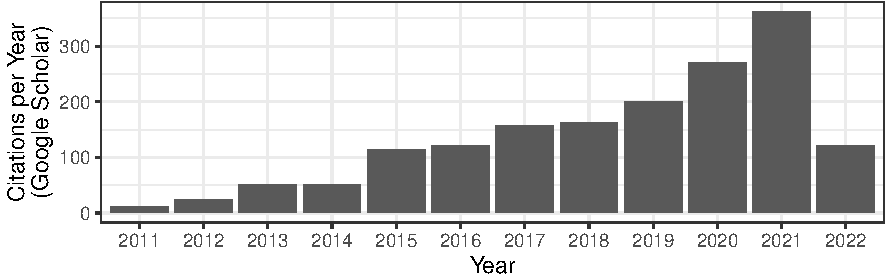
\includegraphics{SchwartzSarah_CV_new_files/figure-latex/unnamed-chunk-3-1} \end{center}

\hypertarget{working-papers-under-revision-or-review}{%
\subsection{\texorpdfstring{\textbf{Working Papers under Revision or
Review}}{Working Papers under Revision or Review}}\label{working-papers-under-revision-or-review}}

\hypertarget{refs_journalspress}{}
\leavevmode\vadjust pre{\hypertarget{ref-ferguson2022}{}}%
\CSLLeftMargin{1. }
\CSLRightInline{Ferguson, M., James, A., Schwartz, S. E., \& Dotterer,
A. (n.d.). Parental microprotections: Testing measurement equivalence
across race/ethnicity. \emph{Family Relations. Special Issue: The
Science of Families: Nurturing Hope, Happiness, and Health}, \emph{Under
Review: 5-23-2022}, Manuscript ID: FR-0154-22.}

\leavevmode\vadjust pre{\hypertarget{ref-mcclain2022interdisc}{}}%
\CSLLeftMargin{2. }
\CSLRightInline{A measure of attitudes toward interdisciplinary
healthcare teams. (n.d.). \emph{Journal of Primary Care and Community
Health}, \emph{Under Review: 3-29-2022}, Manuscript ID: JPC-22-0073.R1.}

\leavevmode\vadjust pre{\hypertarget{ref-golson2022racialgender}{}}%
\CSLLeftMargin{3. }
\CSLRightInline{Racial and gender bias in school psychologists' special
education classification considerations. (n.d.). \emph{School
Psychology}, \emph{Under Review: 3-5-2022}.}

\leavevmode\vadjust pre{\hypertarget{ref-haverkamp2022app}{}}%
\CSLLeftMargin{4. }
\CSLRightInline{Haverkamp, C., Golson, M., Schwartz, S. E., \& McClain,
M. (n.d.). An app-based early academic skills intervention for children
with autism. \emph{Journal of Applied School Psychology}, \emph{Under
Review: 2-24-2022}, Manuscript ID: WAPP-2022-1042.}

\leavevmode\vadjust pre{\hypertarget{ref-mcclain2022scips}{}}%
\CSLLeftMargin{5. }
\CSLRightInline{Golson, M., Harris, B., Schwartz, S. E., Ficklin, E., \&
McClain, M. (n.d.). Caregiver perceptions of social communication and
interaction: Development and validation of the SCIPS. \emph{Autism
Research}, \emph{Under Review: 2-24-2022}.}

\leavevmode\vadjust pre{\hypertarget{ref-Benallie2022life}{}}%
\CSLLeftMargin{6. }
\CSLRightInline{Benallie, K. J., Benney, C. M., McClain, M. B.,
Schwartz, S. E., \& Bakner, K. E. (n.d.). Life satisfaction in children
with and without disabilities, to school mental health.
\emph{Contemporary School Psychology}, \emph{Under Review: 3-14-2022},
Manuscript ID: CASP-D-21-00071R1.}

\leavevmode\vadjust pre{\hypertarget{ref-mcclain2022noise}{}}%
\CSLLeftMargin{7. }
\CSLRightInline{McClain, M. B., Yoho, S. E., B, D. R., Haverkamp, C. R.,
\& Schwartz, S. E. (n.d.). Reading skills and background noise in
autistic and non-autistic children: A pilot study. \emph{Contemporary
School Psychology}, \emph{Under Review: 4-22-2022}, Manuscript ID:
LSHSS-21-00147R1.}

\leavevmode\vadjust pre{\hypertarget{ref-McClain2021vineland}{}}%
\CSLLeftMargin{8. }
\CSLRightInline{McClain, M. B., Schwartz, S. E., Bera, J., Serang, S.,
Farmer, R., Harris, B., \& Golson, M. E. (n.d.). Vineland-3 measurement
non-invariance in children with and without intellectual and
developmental disabilities. \emph{American Journal on Intellectual and
Developmental Disabilities}, \emph{Under Review: 2-7-2022}, Manuscript
ID: AJIDD-D-21-00075R1.}

\leavevmode\vadjust pre{\hypertarget{ref-Orellana2021}{}}%
\CSLLeftMargin{9. }
\CSLRightInline{Orellana, C., Schwartz, S. E., Juth, S., Ding, G., Wada,
R., Hancock, A., \& Gillam, R. B. (n.d.). Working memory and syntactic
processing bilingual and monolingual children. \emph{PLOS ONE},
\emph{Under Review: 1-5-2021}, Manuscript ID: PONE-D-21-00420.}

\leavevmode\vadjust pre{\hypertarget{ref-Fox2021}{}}%
\CSLLeftMargin{10. }
\CSLRightInline{Fox, C. B., Jones, S., Gillam, S. L., Schwartz, S. E.,
\& Gillam, R. (n.d.). Removing barriers to language sample analysis:
Computer automated microstructure scoring (CAMS). \emph{Computer Speech
\& Language}, Under Review: 1-20-2021.}

\leavevmode\vadjust pre{\hypertarget{ref-jex2021}{}}%
\CSLLeftMargin{11. }
\CSLRightInline{Jex, E., Morgan, R., \& Schwartz, S. E. (n.d.). Special
education teachers' perceptions regarding use of transition assessment
for students with severe disabilities. \emph{Research and Practice for
Persons with Severe Disabilities}, \emph{Under Review: 8-11-2021},
Manuscript ID: RPSD-21-08-073.}

\leavevmode\vadjust pre{\hypertarget{ref-haverkamp2021mindfull}{}}%
\CSLLeftMargin{12. }
\CSLRightInline{Haverkamp, C., Schwartz, S. E., Strait, G., Strait, J.,
\& Benney, C. (n.d.). Improving the efficiency and accessibility of
mindfulness meditation: A randomized controlled trial. \emph{Journal of
American College Health}, \emph{Under Review: 6-18-2019}, Manuscript ID:
JACH-2019-06-0270.}

\vspace{7mm}

\hypertarget{refereed-journal-papers---2022}{%
\subsection{\texorpdfstring{\textbf{Refereed Journal Papers -
2022}}{Refereed Journal Papers - 2022}}\label{refereed-journal-papers---2022}}

\hypertarget{refs_journals2022}{}
\leavevmode\vadjust pre{\hypertarget{ref-Reuveni2022cannabinoids}{}}%
\CSLLeftMargin{1. }
\CSLRightInline{Reuveni, N., Carlson, C., Schwartz, S. E., Meter, D.,
Barrett, T., \& Freeman, S. M. (n.d.). The antidepressant and anxiolytic
effect of cannabinoids in chronic unpredictable stress: A preclinical
systematic review and meta-analysis. \emph{Research and Practice for
Persons with Severe Disabilities}, \emph{Under Review: 8-9-2021},
Reference Number: 2021TP001023.}

\leavevmode\vadjust pre{\hypertarget{ref-fox2022lluna}{}}%
\CSLLeftMargin{2. }
\CSLRightInline{Fox, C., Jones, S., Gillam, S., Israelsen-Augenstein,
M., Schwartz, S. E., \& Gillam, R. B. (n.d.). Automated
progress-monitoring through literate language use in narrative
assessment (LLUNA). \emph{Frontiers in Psychology}, \emph{Technology to
the Rescue: Automating Language Sample Analyses for the Assessment and
Treatment of Communication Disorders across the Life-span}, Manuscript
Published: May 16, 2022.}

\leavevmode\vadjust pre{\hypertarget{ref-Ferguson2022parsex}{}}%
\CSLLeftMargin{3. }
\CSLRightInline{Ferguson, M. M., Dotterer, A. M., Schwartz, S. E., \&
Bradford, K. (2022). Parental sexual communication self-efficacy with
toddlers and young children: An active learning intervention. \emph{Sex
Education}, \emph{0}(0), 1--19.
\url{https://doi.org/10.1080/14681811.2022.2034612}}

\leavevmode\vadjust pre{\hypertarget{ref-golson2022current}{}}%
\CSLLeftMargin{4. }
\CSLRightInline{Golson, M. E., Benallie, K. J., Benney, C. M., Schwartz,
S. E., McClain, M. B., \& Harris, B. (2022). Current state of autism
knowledge in the general population of the united states. \emph{Research
in Autism Spectrum Disorders}, \emph{90}, 101886.}

\hypertarget{refereed-journal-papers---2021}{%
\subsection{\texorpdfstring{\textbf{Refereed Journal Papers -
2021}}{Refereed Journal Papers - 2021}}\label{refereed-journal-papers---2021}}

\hypertarget{refs_journals2021}{}
\leavevmode\vadjust pre{\hypertarget{ref-murray2021sleep}{}}%
\CSLLeftMargin{1. }
\CSLRightInline{Murray, J., Gonzalez, H. L., Schwartz, S. E., Rattinger,
G. B., Liu, Y., Hammond, A. G., Kauzor, K. E., Drewel, M., \& Tschanz,
J. T. (2021). Sleep disturbance and association with cognitive and
functional trajectories in all cause dementia: The cache county dementia
progression study. \emph{Alzheimer's \& Dementia}, \emph{17}, e054131.}

\leavevmode\vadjust pre{\hypertarget{ref-pitt2021long}{}}%
\CSLLeftMargin{2. }
\CSLRightInline{Pitt, C., Muñoz, K., Schwartz, S., \& Kunz, J. M.
(2021). The long-term stability of the electrical stapedial reflex
threshold. \emph{Otology \& Neurotology}, \emph{42}(1), 188--196.}

\leavevmode\vadjust pre{\hypertarget{ref-mcclain2021effective}{}}%
\CSLLeftMargin{3. }
\CSLRightInline{McClain, M. B., Haverkamp, C. R., Benallie, K. J.,
Schwartz, S. E., \& Simonsmeier, V. (2021). How effective are reading
comprehension interventions for children with ASD? A meta-analysis of
single-case design studies. \emph{School Psychology}, \emph{36}(2),
107.}

\leavevmode\vadjust pre{\hypertarget{ref-wengreen2021randomized}{}}%
\CSLLeftMargin{4. }
\CSLRightInline{Wengreen, H. J., Joyner, D., Kimball, S. S., Schwartz,
S. E., \& Madden, G. J. (2021). A randomized controlled trial evaluating
the FIT game's efficacy in increasing fruit and vegetable consumption.
\emph{Nutrients}, \emph{13}(8), 2646.}

\leavevmode\vadjust pre{\hypertarget{ref-england2021relationship}{}}%
\CSLLeftMargin{5. }
\CSLRightInline{England, D., Ruddy, K. L., Dakin, C. J., Schwartz, S.
E., Butler, B., \& Bolton, D. A. (2021). Relationship between speed of
response inhibition and ability to suppress a step in midlife and older
adults. \emph{Brain Sciences}, \emph{11}(5), 643.}

\leavevmode\vadjust pre{\hypertarget{ref-mcclain2021differential}{}}%
\CSLLeftMargin{6. }
\CSLRightInline{McClain, M. B., Harris, B., Schwartz, S. E., \& Golson,
M. E. (2021). Brief report: Differential item and test functioning of
the autism spectrum rating scales: A follow-up evaluation in a diverse,
nonclinical sample. \emph{Journal of Psychoeducational Assessment},
\emph{39}(2), 247--257.}

\leavevmode\vadjust pre{\hypertarget{ref-golson2021influences}{}}%
\CSLLeftMargin{7. }
\CSLRightInline{Golson, M. E., Haverkamp, C. R., McClain, M. B.,
Schwartz, S. E., Ha, J., Harris, B., \& Benallie, K. J. (2021).
Influences of student race/ethnicity and gender on autism special
education classification considerations. \emph{Autism},
13623613211050440.}

\leavevmode\vadjust pre{\hypertarget{ref-aller2021measuring}{}}%
\CSLLeftMargin{8. }
\CSLRightInline{Aller, T. B., Fauth, E. B., Novak, J. R., \& Schwartz,
S. E. (2021). Measuring mental health literacy: Development of the
mental health awareness and advocacy assessment tool. \emph{Journal of
MultiDisciplinary Evaluation}, \emph{17}(39), 15--31.}

\vspace{7mm}

\hypertarget{refereed-journal-papers---2020}{%
\subsection{\texorpdfstring{\textbf{Refereed Journal Papers -
2020}}{Refereed Journal Papers - 2020}}\label{refereed-journal-papers---2020}}

\hypertarget{refs_journals2020}{}
\leavevmode\vadjust pre{\hypertarget{ref-bringhurst2020wingate}{}}%
\CSLLeftMargin{1. }
\CSLRightInline{Bringhurst, R. F., Wagner, D. R., \& Schwartz, S.
(2020). Wingate anaerobic test reliability on the velotron with ice
hockey players. \emph{The Journal of Strength \& Conditioning Research},
\emph{34}(6), 1716--1722.}

\leavevmode\vadjust pre{\hypertarget{ref-mcclain2020evaluation}{}}%
\CSLLeftMargin{2. }
\CSLRightInline{McClain, M. B., Harris, B., Schwartz, S. E., \& Golson,
M. E. (2020). Evaluation of the autism spectrum rating scales in a
diverse, nonclinical sample. \emph{Journal of Psychoeducational
Assessment}, \emph{38}(6), 740--752.}

\leavevmode\vadjust pre{\hypertarget{ref-buenabad2020cluster}{}}%
\CSLLeftMargin{3. }
\CSLRightInline{Buenabad, N. G. A., Ramos, R. S., Schwartz, S., López,
M. L. G., Juárez, A. D. D., Gallegos, A. B. O., Ortega, T. G. G., Pérez,
L. V., Icaza, M. E. M.-M., Rodrı́guez, M. M. D.others. (2020). Cluster
randomized trial of a multicomponent school-based program in mexico to
prevent behavioral problems and develop social skills in children.
\emph{Child \& Youth Care Forum}, \emph{49}, 343--364.}

\leavevmode\vadjust pre{\hypertarget{ref-harris2020knowledge}{}}%
\CSLLeftMargin{4. }
\CSLRightInline{Harris, B., McClain, M. B., Schwartz, S., \& Haverkamp,
C. R. (2020). Knowledge of autism spectrum disorder among school
psychology graduate students. \emph{Contemporary School Psychology},
1--9.}

\leavevmode\vadjust pre{\hypertarget{ref-mcclain2020asksp}{}}%
\CSLLeftMargin{5. }
\CSLRightInline{McClain, M. B., Harris, B., Haverkamp, C. R., Golson, M.
E., \& Schwartz, S. E. (2020). The ASKSP revised (ASKSP-r) as a measure
of ASD knowledge for professional populations. \emph{Journal of Autism
and Developmental Disorders}, \emph{50}(3), 998--1006.}

\leavevmode\vadjust pre{\hypertarget{ref-mcclain2020school}{}}%
\CSLLeftMargin{6. }
\CSLRightInline{McClain, M. B., Shahidullah, J. D., Mezher, K. R.,
Haverkamp, C. R., Benallie, K. J., \& Schwartz, S. E. (2020).
School-clinic care coordination for youth with ASD: A national survey of
school psychologists. \emph{Journal of Autism and Developmental
Disorders}, \emph{50}(9), 3081--3091.}

\leavevmode\vadjust pre{\hypertarget{ref-vazquez2020innovative}{}}%
\CSLLeftMargin{7. }
\CSLRightInline{Vázquez, A. L., Rodrı́guez, M. M. D., Barrett, T. S.,
Schwartz, S., Buenabad, N. G. A., Gamiño, M. N. B., López, M. de L. G.,
\& Velázquez, J. A. V. (2020). Innovative identification of substance
use predictors: Machine learning in a national sample of mexican
children. \emph{Prevention Science}, \emph{21}(2), 171--181.}

\leavevmode\vadjust pre{\hypertarget{ref-benallie2020validation}{}}%
\CSLLeftMargin{8. }
\CSLRightInline{Benallie, K. J., McClain, M. B., Harris, B., \&
Schwartz, S. E. (2020). Validation of the ASKSG with a parent sample in
the united states. \emph{Journal of Autism and Developmental Disorders},
\emph{50}(12), 4557--4565.}

\leavevmode\vadjust pre{\hypertarget{ref-torres2020reactions}{}}%
\CSLLeftMargin{9. }
\CSLRightInline{Torres, L., Reveles, A. K., Mata-Greve, F., Schwartz,
S., \& Domenech Rodriguez, M. M. (2020). Reactions to witnessing ethnic
microaggressions: An experimental study. \emph{Journal of Social and
Clinical Psychology}, \emph{39}(2), 141--164.}

\leavevmode\vadjust pre{\hypertarget{ref-nagaraj2020auditory}{}}%
\CSLLeftMargin{10. }
\CSLRightInline{Nagaraj, N. K., Magimairaj, B. M., \& Schwartz, S.
(2020). Auditory distraction in school-age children relative to
individual differences in working memory capacity. \emph{Attention,
Perception, \& Psychophysics}, \emph{82}, 3581--3593.}

\vspace{7mm}

\hypertarget{refereed-journal-papers---2019}{%
\subsection{\texorpdfstring{\textbf{Refereed Journal Papers -
2019}}{Refereed Journal Papers - 2019}}\label{refereed-journal-papers---2019}}

\hypertarget{refs_journals2019}{}
\leavevmode\vadjust pre{\hypertarget{ref-wagner2019mode}{}}%
\CSLLeftMargin{1. }
\CSLRightInline{Wagner, D. R., Thompson, B. J., Anderson, D. A., \&
Schwartz, S. (2019). A-mode and b-mode ultrasound measurement of fat
thickness: A cadaver validation study. \emph{European Journal of
Clinical Nutrition}, \emph{73}(4), 518--523.}

\leavevmode\vadjust pre{\hypertarget{ref-rattinger2019neuropsychiatric}{}}%
\CSLLeftMargin{2. }
\CSLRightInline{Rattinger, G. B., Sanders, C. L., Vernon, E., Schwartz,
S., Behrens, S., Lyketsos, C. G., \& Tschanz, J. T. (2019).
Neuropsychiatric symptoms in patients with dementia and the longitudinal
costs of informal care in the cache county population. \emph{Alzheimer's
\& Dementia: Translational Research \& Clinical Interventions},
\emph{5}, 81--88.}

\leavevmode\vadjust pre{\hypertarget{ref-bolton2019motor}{}}%
\CSLLeftMargin{3. }
\CSLRightInline{Bolton, D. A., Cole, D. M., Butler, B., Mansour, M.,
Rydalch, G., McDannald, D. W., \& Schwartz, S. E. (2019). Motor
preparation for compensatory reach-to-grasp responses when viewing a
wall-mounted safety handle. \emph{Cortex}, \emph{117}, 135--146.}

\leavevmode\vadjust pre{\hypertarget{ref-bolton2019priming}{}}%
\CSLLeftMargin{4. }
\CSLRightInline{Bolton, D. A., Schwartz, S. E., Mansour, M., Rydalch,
G., \& McDannald, D. W. (2019). Priming of grasping muscles when viewing
a safety handle is diminished with age. \emph{Maturitas}, \emph{121},
7--12.}

\leavevmode\vadjust pre{\hypertarget{ref-montgomery2019comparison}{}}%
\CSLLeftMargin{5. }
\CSLRightInline{Montgomery, J. W., Gillam, R. B., Evans, J. L.,
Schwartz, S., \& Fargo, J. D. (2019). A comparison of the storage-only
deficit and joint mechanism deficit hypotheses of the verbal working
memory storage capacity limitation of children with developmental
language disorder. \emph{Journal of Speech, Language, and Hearing
Research}, \emph{62}(10), 3808--3825.}

\leavevmode\vadjust pre{\hypertarget{ref-matyi2019lifetime}{}}%
\CSLLeftMargin{6. }
\CSLRightInline{Matyi, J. M., Rattinger, G. B., Schwartz, S., Buhusi,
M., \& Tschanz, J. T. (2019). Lifetime estrogen exposure and cognition
in late life: The cache county study. \emph{Menopause (New York, NY)},
\emph{26}(12), 1366.}

\leavevmode\vadjust pre{\hypertarget{ref-kauzor2019p1}{}}%
\CSLLeftMargin{7. }
\CSLRightInline{Kauzor, K. E., Schwartz, S., Tubbs, Z., Hammond, A. G.,
\& Tschanz, J. T. (2019). P1-478: PATTERNS OF NEUROPSYCHIATRIC SYMPTOMS
AND SURVIVAL AMONG OLDER ADULTS WITH VARIOUS SUBTYPES OF DEMENTIA: THE
CACHE COUNTY DEMENTIA PROGRESSION STUDY. \emph{Alzheimer's \& Dementia},
\emph{15}, P452--P452.}

\leavevmode\vadjust pre{\hypertarget{ref-mcclain2019brief}{}}%
\CSLLeftMargin{8. }
\CSLRightInline{McClain, M. B., Harris, B., Schwartz, S. E., Benallie,
K. J., Golson, M. E., \& Benney, C. M. (2019). Brief report: Development
and validation of the autism spectrum knowledge scale general population
version: Preliminary analyses. \emph{Journal of Autism and Developmental
Disorders}, \emph{49}(7), 3007--3015.}

\leavevmode\vadjust pre{\hypertarget{ref-vazquez2019early}{}}%
\CSLLeftMargin{9. }
\CSLRightInline{Vázquez, A. L., Domenech Rodrı́guez, M. M., Schwartz, S.,
Amador Buenabad, N. G., Bustos Gamiño, M. N., Gutierrez López, M. de L.,
\& Villatoro Velázquez, J. A. (2019). Early adolescent substance use in
a national sample of mexican youths: Demographic characteristics that
predict use of alcohol, tobacco, and other drugs. \emph{Journal of
Latinx Psychology}, \emph{7}(4), 273.}

\leavevmode\vadjust pre{\hypertarget{ref-vazquez2019authors}{}}%
\CSLLeftMargin{10. }
\CSLRightInline{Vázquez, A. L., Rodrı́guez, M. M. D., Schwartz, S. E.,
Buenabad, N. G. A., Gamiño, M. N. B., López, M. de L. G., Velázquez, J.
A. V., Vázquez, A., Domenech Rodrı́guez, M., Schwartz, S.others. (2019).
\emph{Authors' permission. The final article will be available, upon
publication, via its DOI}.}

\vspace{7mm}

\hypertarget{refereed-journal-papers---2018}{%
\subsection{\texorpdfstring{\textbf{Refereed Journal Papers -
2018}}{Refereed Journal Papers - 2018}}\label{refereed-journal-papers---2018}}

\hypertarget{refs_journals2018}{}
\leavevmode\vadjust pre{\hypertarget{ref-montgomery2018}{}}%
\CSLLeftMargin{1. }
\CSLRightInline{Montgomery, J. W., Evans, J. L., Fargo, J. D., Schwartz,
S. E., \& Gillam, R. B. (2018). Structural relationship between
cognitive processing and syntactic sentence comprehension in children
with and without developmental language disorder. \emph{Journal of
Speech, Language, and Hearing Research}, \emph{61}(12), 2950--2976.}

\leavevmode\vadjust pre{\hypertarget{ref-sanders2018}{}}%
\CSLLeftMargin{2. }
\CSLRightInline{Sanders, C. L., Wengreen, H. J., Schwartz, S. E.,
Behrens, S. J., Corcoran, C., Lyketsos, C. G., \& Tschanz, J. T. (2018).
Nutritional status is associated with severe dementia and mortality.
\emph{Alzheimer Disease \& Associated Disorders}, \emph{32}(4),
298--304.}

\leavevmode\vadjust pre{\hypertarget{ref-behrens2018}{}}%
\CSLLeftMargin{3. }
\CSLRightInline{Behrens, S., Rattinger, G. B., Schwartz, S. E., Matyi,
J., Sanders, C., DeBerard, M. S., Lyketsos, C. G., \& Tschanz, J. T.
(2018). Use of FDA approved medications for alzheimer's disease in mild
dementia is associated with reduced informal costs of care.
\emph{International Psychogeriatrics}, \emph{30}(10), 1499--1507.}

\leavevmode\vadjust pre{\hypertarget{ref-bringhurst2018}{}}%
\CSLLeftMargin{4. }
\CSLRightInline{Bringhurst, R. F., Wagner, D. R., \& Schwartz, S.
(2018). Wingate anaerobic test reliability on the velotron with ice
hockey players. \emph{Journal of Strength and Conditioning Research}.
\url{https://doi.org/10.1519/JSC.0000000000002458}}

\vspace{7mm}

\hypertarget{refereed-journal-papers---2017-and-prior}{%
\subsection{\texorpdfstring{\textbf{Refereed Journal Papers - 2017 and
Prior}}{Refereed Journal Papers - 2017 and Prior}}\label{refereed-journal-papers---2017-and-prior}}

\hypertarget{refs_journals2017}{}
\leavevmode\vadjust pre{\hypertarget{ref-rattinger2016closer}{}}%
\CSLLeftMargin{1. }
\CSLRightInline{Rattinger, G. B., Fauth, E. B., Behrens, S., Sanders,
C., Schwartz, S. E., Norton, M. C., Corcoran, C., Mullins, C. D.,
Lyketsos, C. G., \& Tschanz, J. T. (2016). Closer caregiver and
care-recipient relationships predict lower informal costs of dementia
care: The cache county dementia progression study. \emph{Alzheimer's \&
Dementia}, \emph{12}(8), 917--924.}

\leavevmode\vadjust pre{\hypertarget{ref-rattinger2016}{}}%
\CSLLeftMargin{2. }
\CSLRightInline{Rattinger, G. B., Fauth, E. B., Behrens, S., Sanders,
C., Schwartz, S. E., Norton, M. C., Corcoran, C., Mullins, C. D.,
Lyketsos, C. G., \& Tschanz, J. T. (2016). Closer caregiver and
care-recipient relationships predict lower informal costs of dementia
care: The cache county dementia progression study. \emph{Alzheimer's \&
Dementia}, \emph{12}(8), 917--924.}

\leavevmode\vadjust pre{\hypertarget{ref-sanders2016}{}}%
\CSLLeftMargin{3. }
\CSLRightInline{Sanders, C., Behrens, S., Schwartz, S. E., Wengreen, H.,
Corcoran, C. D., Lyketsos, C. G., \& Tschanz, J. T. (2016). Nutritional
status is associated with faster cognitive decline and worse functional
impairment in the progression of dementia: The cache county dementia
progression study 1. \emph{Journal of Alzheimer's Disease},
\emph{52}(1), 33--42.}

\leavevmode\vadjust pre{\hypertarget{ref-rattinger2015}{}}%
\CSLLeftMargin{4. }
\CSLRightInline{Rattinger, G. B., Schwartz, S. E., Mullins, C. D.,
Corcoran, C., Zuckerman, I. H., Sanders, C., Norton, M. C., Fauth, E.
B., Leoutsakos, J.-M. S., Lyketsos, C. G.others. (2015). Dementia
severity and the longitudinal costs of informal care in the cache county
population. \emph{Alzheimer's \& Dementia}, \emph{11}(8), 946--954.
\url{https://doi.org/10.1016/j.jalz.2014.11.004}}

\leavevmode\vadjust pre{\hypertarget{ref-peters2015}{}}%
\CSLLeftMargin{5. }
\CSLRightInline{Peters, M. E., Schwartz, S. E., Han, D., Rabins, P. V.,
Steinberg, M., Tschanz, J. T., \& Lyketsos, C. G. (2015).
Neuropsychiatric symptoms as predictors of progression to severe
alzheimer's dementia and death: The cache county dementia progression
study. \emph{American Journal of Psychiatry}, \emph{172}(5), 460--465.}

\leavevmode\vadjust pre{\hypertarget{ref-hatch2015}{}}%
\CSLLeftMargin{6. }
\CSLRightInline{Hatch, D. J., Schwartz, S. E., \& Norton, M. C. (2015).
Depression and antidepressant use moderate association between widowhood
and alzheimer's disease. \emph{International Journal of Geriatric
Psychiatry}, \emph{30}(3), 292--299.}

\leavevmode\vadjust pre{\hypertarget{ref-gurgel2014}{}}%
\CSLLeftMargin{7. }
\CSLRightInline{Gurgel, R. K., Ward, P. D., Schwartz, S. E., Norton, M.
C., Foster, N. L., \& Tschanz, J. T. (2014). Relationship of hearing
loss and dementia: A prospective, population-based study. \emph{Otology
\& Neurotology: Official Publication of the American Otological Society,
American Neurotology Society {[}and{]} European Academy of Otology and
Neurotology}, \emph{35}(5), 775.}

\leavevmode\vadjust pre{\hypertarget{ref-rabins2013}{}}%
\CSLLeftMargin{8. }
\CSLRightInline{Rabins, P. V., Schwartz, S. E., Black, B. S., Corcoran,
C., Fauth, E., Mielke, M., Christensen, J., Lyketsos, C., \& Tschanz, J.
(2013). Predictors of progression to severe alzheimer's disease in an
incidence sample. \emph{Alzheimer's \& Dementia}, \emph{9}(2),
204--207.}

\leavevmode\vadjust pre{\hypertarget{ref-fauth2013}{}}%
\CSLLeftMargin{9. }
\CSLRightInline{Fauth, E. B., Schwartz, S. E., Tschanz, J. T., Østbye,
T., Corcoran, C., \& Norton, M. C. (2013). Baseline disability in
activities of daily living predicts dementia risk even after controlling
for baseline global cognitive ability and depressive symptoms.
\emph{International Journal of Geriatric Psychiatry}, \emph{28}(6),
597--606.}

\leavevmode\vadjust pre{\hypertarget{ref-tschanz2013}{}}%
\CSLLeftMargin{10. }
\CSLRightInline{Tschanz, J., Pfister, R., Steffens, D., Corcoran, C.,
Smith, K., Østbye, T., Schwartz, S., Welsh-Bohmer, K., \& M, N. (2013).
Stressful events in late-life: Effects on cogni-tive decline. The cache
county study. \emph{International Journal of Geriatric Psychiatry},
\emph{28}(8), 820--830.}

\leavevmode\vadjust pre{\hypertarget{ref-norton2011}{}}%
\CSLLeftMargin{11. }
\CSLRightInline{Norton, M. C., Smith, K. R., Østbye, T., Tschanz, J. A.
T., Schwartz, S. E., Corcoran, C., Breitner, J. C., Steffens, D. C.,
Skoog, I., Rabins, P. V.others. (2011). Early parental death and
remarriage of widowed parents as risk factors for alzheimer disease: The
cache county study. \emph{The American Journal of Geriatric Psychiatry},
\emph{19}(9), 814--824.}

\leavevmode\vadjust pre{\hypertarget{ref-tschanz2011}{}}%
\CSLLeftMargin{12. }
\CSLRightInline{Tschanz, J. T., Corcoran, C. D., Schwartz, S. E.,
Treiber, K., Green, R. C., Norton, M. C., Mielke, M. M., Piercy, K.,
Steinberg, M., Rabins, P. V.others. (2011). Progression of cognitive,
functional, and neuropsychiatric symptom domains in a population cohort
with alzheimer dementia: The cache county dementia progression study.
\emph{The American Journal of Geriatric Psychiatry}, \emph{19}(6),
532--542.}

\leavevmode\vadjust pre{\hypertarget{ref-norton2010}{}}%
\CSLLeftMargin{13. }
\CSLRightInline{Norton, M. C., Smith, K. R., Østbye, T., Tschanz, J. T.,
Corcoran, C., Schwartz, S. E., Piercy, K. W., Rabins, P. V., Steffens,
D. C., Skoog, I.others. (2010). Greater risk of dementia when spouse has
dementia? The cache county study: {[}See editorial comments by dr. Peter
p. Vitaliano, pp 976--978{]}. \emph{Journal of the American Geriatrics
Society}, \emph{58}(5), 895--900.}

\leavevmode\vadjust pre{\hypertarget{ref-norton2009}{}}%
\CSLLeftMargin{14. }
\CSLRightInline{Norton, M. C., Smith, K. R., Ostbye, T., Tschanz, J. T.,
Corcoran, C., Schwartz, S. E., Piercy, K. W., Rabins, P. V., Steffens,
D. C., Breitner, J. C.others. (2009). Spousal dementia caregiving as a
risk factor for incident dementia. \emph{Alzheimer's \& Dementia: The
Journal of the Alzheimer's Association}, \emph{5}(4), 380--381.}

\clearpage

\hypertarget{papers-in-refereed-conference-proceedings}{%
\subsection{\texorpdfstring{\textbf{Papers in Refereed Conference
Proceedings}}{Papers in Refereed Conference Proceedings}}\label{papers-in-refereed-conference-proceedings}}

\hypertarget{refs_proceedings}{}
\leavevmode\vadjust pre{\hypertarget{ref-buenabad2020cluster}{}}%
\CSLLeftMargin{1. }
\CSLRightInline{Buenabad, N. G. A., Ramos, R. S., Schwartz, S., López,
M. L. G., Juárez, A. D. D., Gallegos, A. B. O., Ortega, T. G. G., Pérez,
L. V., Icaza, M. E. M.-M., Rodrı́guez, M. M. D.others. (2020). Cluster
randomized trial of a multicomponent school-based program in mexico to
prevent behavioral problems and develop social skills in children.
\emph{Child \& Youth Care Forum}, \emph{49}, 343--364.}

\leavevmode\vadjust pre{\hypertarget{ref-behrens2014agitation}{}}%
\CSLLeftMargin{2. }
\CSLRightInline{Behrens, S., Rattinger, G., Schwartz, S., Lyketsos, C.,
\& Tschanz, J. (2014). AGITATION IN DEMENTIA IS ASSOCIATED WITH WORSE
CAREGIVER HEALTH OVER TIME: THE CACHE COUNTY STUDY.
\emph{GERONTOLOGIST}, \emph{54}, 42--42.}

\leavevmode\vadjust pre{\hypertarget{ref-rattinger2013caregiver}{}}%
\CSLLeftMargin{3. }
\CSLRightInline{Rattinger, G., Schwartz, S., Sanders, C., Corcoran, C.,
Fauth, E., Norton, M., Lyketsos, C., \& Tschanz, J. (2013). HOW DO
CAREGIVER RELATIONSHIP CLOSENESS AND COPING STRATEGIES AFFECT THE COSTS
OF DEMENTIA CARE? \emph{GERONTOLOGIST}, \emph{53}, 114--115.}

\leavevmode\vadjust pre{\hypertarget{ref-smith2011dementia}{}}%
\CSLLeftMargin{4. }
\CSLRightInline{Smith, K., Hanson, H., Ostbye, T., Tschanz, J.,
Schwartz, S., Corcoran, C., \& Norton, M. (2011). DEMENTIA AND THE RISK
ASSOCIATED WITH MEDICAL CO-MORBIDITIES: RESULTS FROM THE CACHE COUNTY
STUDY LINKED TO MEDICARE CLAIMS. \emph{GERONTOLOGIST}, \emph{51},
94--94.}

\leavevmode\vadjust pre{\hypertarget{ref-fauth2011baseline}{}}%
\CSLLeftMargin{5. }
\CSLRightInline{Fauth, E., Schwartz, S., Smith, K., Tschanz, J., Ostbye,
T., Corcoran, C., \& Norton, M. (2011). BASELINE FUNCTIONAL DISABILITY
PREDICTS DEMENTIA RISK EVEN AFTER CONTROLLING FOR COGNITIVE STATUS.
\emph{GERONTOLOGIST}, \emph{51}, 36--37.}

\leavevmode\vadjust pre{\hypertarget{ref-bradford2010timing}{}}%
\CSLLeftMargin{6. }
\CSLRightInline{Bradford, D., Smith, K., Schwartz, S., Tschanz, J.,
Ostbye, T., Corcoran, C., Welsh-Bohmer, K., \& Norton, M. (2010). TIMING
OF OFFSPRING DEATH IN PARENTS'LIVES AND LATE-LIFE COGNITIVE DECLINE. THE
CACHE COUNTY STUDY. \emph{GERONTOLOGIST}, \emph{50}, 462--462.}

\leavevmode\vadjust pre{\hypertarget{ref-orsulic2010individuals}{}}%
\CSLLeftMargin{7. }
\CSLRightInline{Orsulic-Jeras, S., Menne, H., Whitlatch, C., Schwartz,
S., \& Johnson, J. (2010). INDIVIDUALS WITH EARLY ONSET DEMENTIA AND
THEIR CAREGIVERS: PROGRAM ACCEPTABILITY AND FEASIBILITY.
\emph{GERONTOLOGIST}, \emph{50}, 66--66.}

\vspace{7mm}

\hypertarget{conference-presentations-coauthored}{%
\subsection{\texorpdfstring{\textbf{Conference Presentations
Coauthored}}{Conference Presentations Coauthored}}\label{conference-presentations-coauthored}}

\hypertarget{refs_confco}{}
\leavevmode\vadjust pre{\hypertarget{ref-vernon2022aaic}{}}%
\CSLLeftMargin{1. }
\CSLRightInline{Vernon, H. L. and S., K.and Gonzalez, Rattinger, G. B.,
Drewel, M., Smith, K. R., DeBerard, M. S., Kauwe, J., Buhusi, M., \& T.,
Tschanz. J. (2022). \emph{Sex differences in risk for alzheimer's
disease with extended maternal and paternal family history and vascular
risk factors. The cache county study.} Poster to be presented at the
Alzheimer's Asociation International Conference.}

\leavevmode\vadjust pre{\hypertarget{ref-Matyi2022aaic}{}}%
\CSLLeftMargin{2. }
\CSLRightInline{Matyi, J., Drewel, M., Schwartz, S. E., Rattinger, G.
B., Gonzalez, H., DeBerard, M. S., Buhusi, M., Lyketsos, C. G., \& T.,
T. J. (2022). \emph{Brain-derived neurotrophic factor genes are
associated with neuropsychiatric symptom progression in dementia. The
cache county dementia progression study.} Abstract accepted for the
Alzheimer's Asociation International Conference.}

\leavevmode\vadjust pre{\hypertarget{ref-holbrook2022asha}{}}%
\CSLLeftMargin{3. }
\CSLRightInline{Holbrook, S., Schwartz, S. E., Barrett, T., \& Gillam,
S. (2022). \emph{Validity and reliability of a novel speech prosody
screening tool for autistic children}. Presentation for the American
Speech-Language-Hearing Association Convention.}

\leavevmode\vadjust pre{\hypertarget{ref-bera2022conf}{}}%
\CSLLeftMargin{4. }
\CSLRightInline{Bera, J., Goldon, M., McClain, M., Farmer, R., Harris,
B., Serang, S., \& Schwartz, S. E. (2022). \emph{Testing measurement
invariance in the vineland 3}. Presented at the Annual Convention of the
National Association of School Psychologists.}

\leavevmode\vadjust pre{\hypertarget{ref-golson2021isa}{}}%
\CSLLeftMargin{5. }
\CSLRightInline{Golson, M. E., McClain, M. B., Schwartz, S. E., Bakner,
K. E., Gabrielsen, T., \& Harris, B. (2021). \emph{Measurement
invariance across gender of the ASRS in a non-clinical diverse sample.}
Poster presented at the virtual meeting of the International Society of
Autism Research Annual Meeting.}

\leavevmode\vadjust pre{\hypertarget{ref-golson2021apa}{}}%
\CSLLeftMargin{6. }
\CSLRightInline{Golson, M. E., McClain, M. B., \& Schwartz, S. E.
(2021). \emph{Measurement invariance of the conners-3.} Poster presented
for the virtual meeting of the American Psychological Association,
Division 16 (School Psychology).}

\leavevmode\vadjust pre{\hypertarget{ref-cole2019poster}{}}%
\CSLLeftMargin{7. }
\CSLRightInline{Cole, D., Butler, B., M, M., Schwartz, S. E., \& Bolton,
D. (2019). \emph{An invisible hand: Automatic preparation for arresting
a fall when viewing a handrail.} Poster presented at the International
Society of Posture; Gait Research World Congress, Ediburgh, Scotland.}

\leavevmode\vadjust pre{\hypertarget{ref-Kauzor2019poster}{}}%
\CSLLeftMargin{8. }
\CSLRightInline{Kauzor, K., Schwartz, S. E., Hammond, A., Tubbs, Z.,
Rattinger, G., \& Tschanz, J. (2019). \emph{Patterns of neuropsychiatric
symptoms and survival among older adults with various subtypes of
dementia. The cache county dementia progression study.} Poster presented
at the Annual Alzheimer's Association International Conference, Los
Angeles, CA.}

\leavevmode\vadjust pre{\hypertarget{ref-benallie2018poster}{}}%
\CSLLeftMargin{9. }
\CSLRightInline{Benallie, K., Benney, C., McClain, M. B., Schwartz, S.
E., Peacock, G., \& Harris, B. (2018). \emph{Autism spectrum knowledge
scale (ASKS): General population version: Development and preliminary
validation.} Poster presented at the Rocky Mountain Psychological
Association annual conference, Denver, Colorado.}

\leavevmode\vadjust pre{\hypertarget{ref-Matyi2018poster}{}}%
\CSLLeftMargin{10. }
\CSLRightInline{Matyi, J., Rattinger, G., Vernon, E., Schwartz, S. E.,
Buhusi, M., \& Tschanz, J. (2018). \emph{Lifetime estrogen exposure is
associated with cognitive status in late life: The cache county study.}
Poster presented at the Annual Gerontological Society of America
conference, Boston, MA.}

\leavevmode\vadjust pre{\hypertarget{ref-vernon2018poster}{}}%
\CSLLeftMargin{11. }
\CSLRightInline{Vernon, E., Behrens, S., Rattinger, G., Schwartz, S. E.,
\& Tschanz, J. (2018). \emph{Use of sleep medications is associated with
poorer cognition in older male adults: The cache county study.} Poster
presented at the Annual Alzheimer's Association International
Conference, Chicago, IL.}

\leavevmode\vadjust pre{\hypertarget{ref-joann2015poster}{}}%
\CSLLeftMargin{12. }
\CSLRightInline{Tschanz, J., Sanders, C., Wengreen, H., E, S. S.,
Behrens, S., Corcoran, C., \& Lyketsos, C. (2015). \emph{Status and
neuropsychiatric symptoms in dementia: The cache county dementia study.}
Poster presented at the Annual Alzheimer's Association International
Conference, Washington, DC.}

\leavevmode\vadjust pre{\hypertarget{ref-rattinger2015poster}{}}%
\CSLLeftMargin{13. }
\CSLRightInline{Rattinger, G., Behrens, S., Schwartz, S., Corcoran, C.,
Piercy, K., Norton, M., Fauth, E., Lyketsos, C., \& Tschanz, J. (2015).
\emph{How do neuropsychiatric symptoms in persons with dementia affect
caregiver physical and mental health over time? The cache county
dementia progression study.} Poster presented at the Annual Alzheimer's
Association International Conference, Washington, DC.}

\leavevmode\vadjust pre{\hypertarget{ref-saunders2015poster}{}}%
\CSLLeftMargin{14. }
\CSLRightInline{Sanders, C., Wengreen, H., Schwartz, S., Behrens, S.,
Corcoran, C., Lyketsos, C., \& Tschanz, J. (2015). \emph{Nutritional
status and neuropsychological functioning in persons with dementi: The
cache county dementia progression study.} Poster presented at the Annual
International Neuropsychological Society Meeting, Denver, CO.}

\leavevmode\vadjust pre{\hypertarget{ref-joann2014poster}{}}%
\CSLLeftMargin{15. }
\CSLRightInline{Tschanz, J., Sanders, C., Wengreen, H., Schwartz, S. E.,
Behrens, S., Corcoran, C., \& Lyketsos, C. (2014). \emph{Nutritional
status and neuropsychiatric symptoms in dementia: The cache county
dementia study.} Paper presented at the Gerontological Society of
America Annual Meeting, Washington, DC.}

\leavevmode\vadjust pre{\hypertarget{ref-behrens2014poster}{}}%
\CSLLeftMargin{16. }
\CSLRightInline{Behrens, S., Rattinger, G., Schwartz, S., Lyketsos, C.,
\& Tschanz, J. (2014). \emph{Agitation in dementia is associated with
worse caregiver health over time: The cache county study.} Poster
presented at the Gerontological Society of America Annual Meeting,
Washington, DC.}

\leavevmode\vadjust pre{\hypertarget{ref-peters2014poster}{}}%
\CSLLeftMargin{17. }
\CSLRightInline{Peters, M., Schwartz, S. E., Han, D., Rabins, P.,
Tschanz, J., \& Lyketsos, C. (2014). \emph{Neuropsychiatric symptoms as
predictors of progression to severe alzheimer's dementia and death: The
cache county study}. Poster presented at the Annual American Association
of Geriatric Psychiatrists, Orlando, FL.}

\leavevmode\vadjust pre{\hypertarget{ref-gail2013oral}{}}%
\CSLLeftMargin{18. }
\CSLRightInline{Rattinger, G., Schwartz, S. E., Sanders, C., Corcoran,
C., Fauth, E., Norton, M., Lyketsos, C., \& Tschanz, J. (2013).
\emph{Effect of caregiver relationship closeness and coping strategies
on costs of care in the cache county dementia progression study cohort.}
Presentation at the Gerontological Society of America Conference, New
Orleans, LA.}

\leavevmode\vadjust pre{\hypertarget{ref-joann2013pres}{}}%
\CSLLeftMargin{19. }
\CSLRightInline{Tschanz, J., Schwartz, S., Gilbert, M., Wanzek, J.,
Sanders, C., Mielke, M., Cocoran, C., Norton, M., \& Lyketsos, C.
(2013). \emph{Vascular factors as predictors of severe dementia and
mortality in alzheimer's disease. The cache county dementia progression
study.} Presentation at the Alzheimer's Association International
Conference on Alzheimer's Disease, Boston, MA.}

\leavevmode\vadjust pre{\hypertarget{ref-gail2013pres}{}}%
\CSLLeftMargin{20. }
\CSLRightInline{Rattinger, G., Schwartz, S. E., Corcoran, C., Zuckerman,
I., Mullins, C., Norton, M., Fauth, E., Leoutsakos, J., Lyketsos, C., \&
Tschanz, J. (2013). \emph{Effect of dementia severity on costs of care
in the cache county dementia progression study cohort.} Presentation at
the Alzheimer's Association International Conference on Alzheimer's
Disease, Boston, MA.}

\leavevmode\vadjust pre{\hypertarget{ref-sanders2013pres}{}}%
\CSLLeftMargin{21. }
\CSLRightInline{Sanders, C., Wengreen, H., Corcoran, C., Schwartz, S.,
Norton, M., Lyektsos, C., \& Tschanz, J. (2013). \emph{Nutritional
status and progression of dementia. The cache county dementia
progression study.} Presentation at the Alzheimer's Association
International Conference on Alzheimer's Disease, Boston, MA.}

\leavevmode\vadjust pre{\hypertarget{ref-wanzek2013pres}{}}%
\CSLLeftMargin{22. }
\CSLRightInline{Wanzek, J., Schwartz, S., Sanders, C., Gilbert, M.,
Munger, R., Marano, C., Mielke, M., Lyketsos, C., \& Tschanz, J. (2013).
\emph{Diabetes and metabolic syndrome in predicting severe dementia,
institutionalization and mortality in a population-based sample of
alzheimer's disease: The cache county dementia progression study.}
Presentation at the Society of Behavioral Medicine Conference, San
Francisco, CA.}

\leavevmode\vadjust pre{\hypertarget{ref-gurgel2013pres}{}}%
\CSLLeftMargin{23. }
\CSLRightInline{Gurgel, R., Ward, D., Schwartz, S. E., Norton, M., \&
Tschanz, J. (2013). \emph{Relationship of hearing loss and dementia: A
prospective, population-based study.} Oral presentation at the American
Otological Society meeting, Orlando, FL.}

\leavevmode\vadjust pre{\hypertarget{ref-beth2012pres}{}}%
\CSLLeftMargin{24. }
\CSLRightInline{Fauth, E., Schwartz, S. E., Norton, M., Piercy, K.,
Lyketsos, C., \& JT, T. (2012). \emph{Do closer relationships between
caregivers and persons with alzheimer's dementia affect the progression
of neuropsychiatric symptoms in the care recipient?} Presentation at the
Gerontological Society of America meeting, San Diego, CA.}

\leavevmode\vadjust pre{\hypertarget{ref-steinberg2012pres}{}}%
\CSLLeftMargin{25. }
\CSLRightInline{S, M., Schwartz, S. E., Tschanz, J., Corcoran, B., C nad
Black, Fauth, E., Mielke, M., Lyketsos, C., \& Rabins, P. (2012).
\emph{Neuropsychiatric symptoms at baseline shorten time to severe
dementia in a population-based sample of incident alzheimer's disease.}
Presentation at the Alzheimer's Association International Conference on
Alzheimer's Disease, Vancouver, B.C.}

\leavevmode\vadjust pre{\hypertarget{ref-buckley2011pres}{}}%
\CSLLeftMargin{26. }
\CSLRightInline{Buckley, T., Corcoran, C., Schwartz, S. E., Breitner,
J., Zandi, P., Norton, M., Deberard, M., Wengreen, H., Foley, B.,
Welsh-Bohmer, K., Lyketsos, C., \& Tschanz, J. (2011). \emph{NSAID use
does not affect dementia progression or survival in alzheimer's disease:
The cache county dementia progression study.} Presentation at the
Alzheimer's Association International Conference on Alzheimer's Disease,
Paris, Frane.}

\leavevmode\vadjust pre{\hypertarget{ref-rabins2011pres}{}}%
\CSLLeftMargin{27. }
\CSLRightInline{Rabins, P., Schwartz, S. E., Tschanz, J., Corcoran, C.,
Black, B., Fauth, E., Mielke, M., \& Lyketsos, C. (2011). \emph{Risk
factors for severe dementia from a population-based sample of incident
alzheimer's disease: The cache county dementia progression study.}
Presentation at the Alzheimer's Association International Conference on
Alzheimer's Disease, Paris, Frane.}

\leavevmode\vadjust pre{\hypertarget{ref-fauth2011pres}{}}%
\CSLLeftMargin{28. }
\CSLRightInline{Fauth, E. B., Schwartz, S. E., Smith, K., Tschanz, J.,
Ostbye, T., Corcoran, C., \& Norton, M. C. (2011). \emph{Baseline
functional disability predicts dementia risk even after controlling for
cognitive status.} Presentation at the Annual Meeting of the
Gerontological Society of America, Boston, MA.}

\leavevmode\vadjust pre{\hypertarget{ref-smith2011pres}{}}%
\CSLLeftMargin{29. }
\CSLRightInline{Smith, K., Hanson, H., Ostbye, T., Tschanz, J.,
Schwartz, S. E., Corcoran, C., \& Norton, M. (2011). \emph{Comorbidity
and risk for dementia using medicare datasets.} Presentation at the
Annual Meeting of the Gerontological Society of America, Boston, MA.}

\leavevmode\vadjust pre{\hypertarget{ref-joann2010pres}{}}%
\CSLLeftMargin{30. }
\CSLRightInline{Tschanz, J., Pfister, R., Steffens, D., Corcoran, C.,
Smith, K., Ostbye, T., Schwartz, S. E., Welsh-Bohmer, K., \& Norton, M.
(2010). \emph{Stressful events in late-life: Effects on cognitive
decline. The cache county study.} Poster presentation at the Annual
Meeting of the Gerontological Society of America, New Orleans, LA.}

\leavevmode\vadjust pre{\hypertarget{ref-snyder2010pres}{}}%
\CSLLeftMargin{31. }
\CSLRightInline{Snyder, C., Smith, C., Lee, S., Norton, M., Piercy, K.,
Fauth, E., Corcoran, C., DeBerard, S., Schwartz, S. E., Morrison, A.,
Rabins, P., Lyketsos, C., \& Tschanz, J. (2010). \emph{Dementia
caregivers and coping strategies: Relationship to health and well-being.
The cache county dementia progression study.} Poster presentation at the
Annual Meeting of the Gerontological Society of America, New Orleans,
LA.}

\leavevmode\vadjust pre{\hypertarget{ref-maria2010pres}{}}%
\CSLLeftMargin{32. }
\CSLRightInline{Norton, M., Bradford, D., Smith, K., Schwartz, S. E.,
Tschanz, J., Ostbye, T., Corcoran, C., \& Welsh-Bohmer, K. (2010).
\emph{Family size moderates the association between offspring death and
rate of cognitive decline. The cache county study.} Poster presentation
at the Annual Meeting of the Gerontological Society of America, New
Orleans, LA.}

\leavevmode\vadjust pre{\hypertarget{ref-brandford2010pres}{}}%
\CSLLeftMargin{33. }
\CSLRightInline{Bradford, D., Smith, K., Schwartz, S. E., Tschanz, J.,
Ostbye, T., Corcoran, C., Welsh-Bohmer, K., \& Norton, M. (2010).
\emph{Timing of offspring death in parents' lives and late-life
cognitive decline. The cache county study.} Poster presentation at the
Annual Meeting of the Gerontological Society of America, New Orleans,
LA.}

\leavevmode\vadjust pre{\hypertarget{ref-maria2009pres}{}}%
\CSLLeftMargin{34. }
\CSLRightInline{Norton, M., Smith, K., Ostbye, T., Tschanz, J.,
Corcoran, C., Schwartz, S. E., Piercy, K., Rabins, P., Steffens, D.,
Breitner, J., \& Welsh-Bohmer, K. (2009). \emph{Spousal dementia
caregiving as a risk factor for incident dementia.} Poster presentation
at the International Conference on Alzheimer's Disease, Vienna,
Austria.}

\leavevmode\vadjust pre{\hypertarget{ref-chris2009pres}{}}%
\CSLLeftMargin{35. }
\CSLRightInline{Corcoran, C., Tschanz, J., Steinberg, M., Schwartz, S.
E., Norton, M., Welsh-Bohmer, K., Breitner, J., \& Lyketsos, C. (2006).
\emph{Longitudinal course of neuropsychiatric symptoms in dementia. The
cache county study.} Poster presentation at the 10th International
Conference on Alzheimer's Disease; Related Disorders, Madrid Spain.}

\vspace{7mm}

\hypertarget{work-not-peer-reviewed}{%
\subsection{\texorpdfstring{\textbf{Work Not Peer
Reviewed}}{Work Not Peer Reviewed}}\label{work-not-peer-reviewed}}

\hypertarget{refs_notpeer}{}
\leavevmode\vadjust pre{\hypertarget{ref-McClain_Harris_Schwartz_Haverkamp_Golson_2019}{}}%
\CSLLeftMargin{1. }
\CSLRightInline{McClain, M. B., Harris, B., Schwartz, S. E., Haverkamp,
C. R., \& Golson, M. (2019). \emph{Development and validation of the
autism spectrum knowledge scale - professional version: Preliminary
analyses}. OSF. \url{https://doi.org/10.17605/OSF.IO/8M9UB}}

\clearpage

\vspace{7mm}

\hypertarget{disertation}{%
\subsection{\texorpdfstring{\textbf{Disertation}}{Disertation}}\label{disertation}}

\hypertarget{refs_student}{}
\leavevmode\vadjust pre{\hypertarget{ref-schwartz2017exact}{}}%
\CSLLeftMargin{1. }
\CSLRightInline{Schwartz, S. E. (2017). \emph{Exact approaches for bias
detection and avoidance with small, sparse, or correlated categorical
data} {[}PhD thesis{]}.}

\vspace{7mm}

\hypertarget{online-ebook}{%
\subsection{\texorpdfstring{\textbf{Online
eBook}}{Online eBook}}\label{online-ebook}}

\hypertarget{refs_ebook}{}
\leavevmode\vadjust pre{\hypertarget{ref-eBook6600}{}}%
\CSLLeftMargin{1. }
\CSLRightInline{Schwartz, S. E., \& Barrett, T. S. (2018).
\emph{Explaining psychological statistcs: A compantion in r}. GitHub.
\url{https://sarbearschwartz.github.io/Quant_I/}}

\leavevmode\vadjust pre{\hypertarget{ref-eBookEncyclopedia}{}}%
\CSLLeftMargin{2. }
\CSLRightInline{Schwartz, S. E., \& Barrett, T. S. (2019).
\emph{Encyclopedia of quantitative methods in r}. GitHub.
\url{https://cehs-research.github.io/eBooks/}}

\clearpage

\hypertarget{directed-student-learning}{%
\section{Directed Student Learning}\label{directed-student-learning}}

\hypertarget{research-assistants-for-the-statistical-consulting-studio}{%
\subsection{\texorpdfstring{\textbf{Research Assistants for the
Statistical Consulting
Studio}}{Research Assistants for the Statistical Consulting Studio}}\label{research-assistants-for-the-statistical-consulting-studio}}

\begin{itemize}
\tightlist
\item
  Demi Culianos, 2020-2021
\item
  Jeremy Haynes, 2019-2020
\item
  Ryan Becker, 2019
\item
  Joseph Jones, 2018-2019
\item
  Morgan Kawamura, 2018
\item
  Fred Hints, 2018
\item
  Andy Craig, 2017-2018
\item
  Tyson Barrett, 2016-2017
\end{itemize}

\vspace{7 mm}

\hypertarget{current-committees}{%
\section{Current Committees}\label{current-committees}}

\hypertarget{doctoral}{%
\subsection{\texorpdfstring{\textbf{DOCTORAL}}{DOCTORAL}}\label{doctoral}}

\nopagebreak
    \cventry{(in progress)}{Stephanie (Crank) Avila}{Psychology - Brain and Cognition}{Utah State University}{}{\begin{itemize}%
\item Language influene on deception and its detection%
\item Expected defense: Spring 2023%
\item Mentor: Dr. Chris Warren%
\end{itemize}}
    \cventry{(in progress)}{Olysola Omisakin}{Sociology}{Utah State University}{}{\begin{itemize}%
\item BMI trajectories in the AddHealth%
\item Mulilevel Modeling with Multiple Imputations%
\item Mentor: Dr. Eric Reither%
\end{itemize}}
    \cventry{(in progress)}{Megan Golson}{Psychology - Combined Program}{Utah State University}{}{\begin{itemize}%
\item ADHD knowledge and its relationship to stigma and treatment decisions among parents%
\item Committee Fromed: June 2021%
\item Mentor: Dr. Maryellen McClain Verdose%
\end{itemize}}
    \cventry{(in progress)}{Demi Culianas}{Psychology}{Utah State University}{}{\begin{itemize}%
\item Disertation Title: TBD%
\item Comprehensive examimation passed: April 2021%
\item Mentor: Dr. Tyson Barrett%
\end{itemize}}
    \cventry{(in progress)}{Jill Ashby Harmon}{Curriculum and Instruction}{Utah State University}{}{\begin{itemize}%
\item Relationships Between School, Teacher, and Feature Characteristics and Teachers’ Access to Features within Digital Curriculum Resources for Mathematics Instruction Reported by Teachers on the Rand Corporation American Instructional Resources Survey (AIRS) 2019%
\item Defended proposal: May 2021%
\item Mentor: Dr. Patricia Moyer-Packenham%
\end{itemize}}
    \cventry{(in progress)}{Chris Johnson}{Statistics}{Utah State University}{}{\begin{itemize}%
\item Comprehensive examimation passed: July 2021%
\item Mentor: Dr. Chris Corcoran%
\end{itemize}}
    \cventry{(in progress)}{Kandice Benalli}{Psychology - Combined Program}{Utah State University}{}{\begin{itemize}%
\item Executive Functioning in Children with ASD and Co-occurring Neurodevelopmental Disorders: A Systematic Review and Quantitative Analysis%
\item Expected defense: 2022 (currently collecting data)%
\item Mentor: Dr. Maryellen McClain Verdose%
\end{itemize}}
    \cventry{(in progress)}{Cassity Havercamp}{Psychology - Combined Program}{Utah State University}{}{\begin{itemize}%
\item App-Based Academic Interventions for Children with Autism Spectrum Disorder%
\item Expected defense: 2022%
\item Mentor: Dr. Maryellen McClain Verdose%
\end{itemize}}

\vspace{7 mm}

\hypertarget{masters}{%
\subsection{\texorpdfstring{\textbf{MASTERS}}{MASTERS}}\label{masters}}

\nopagebreak
    \cventry{(in progress)}{Ben Juarez}{Psychology - Clinical Counseling}{Utah State University}{}{\begin{itemize}%
\item CRIES-8 Validation with Latinx Youth%
\item Proposal defense: April 13, 2022%
\item Mentor: Dr. Melanie Domenech Rodriguez%
\end{itemize}}

\vspace{7 mm}

\hypertarget{past-committees}{%
\section{Past Committees}\label{past-committees}}

\hypertarget{chair}{%
\subsection{\texorpdfstring{\textbf{CHAIR}}{CHAIR}}\label{chair}}

\nopagebreak
    \cventry{May 2021}{Amanda Hagman}{Psychology, Socio-Epidemiology Program}{Utah State University}{}{\begin{itemize}%
\item Substance Misuse Transitions Between Adolescence Young Adulthood: Impacts on Young Adult Self-sufficiency%
\item https://digitalcommons.usu.edu/etd/8050/%
\end{itemize}}

\vspace{7 mm}

\hypertarget{doctoral-1}{%
\subsection{\texorpdfstring{\textbf{DOCTORAL}}{DOCTORAL}}\label{doctoral-1}}

\nopagebreak
    \cventry{Dec 2021}{Carly Fox}{Communicative Disorders and Deaf Education}{Utah State University}{}{\begin{itemize}%
\item An Investigation into the Feasibility of Streamlining Language Sample Analysis through Computer-Automated Transcription and Scoring%
\item Master's degree awarded: May 2021%
\item Mentor: Dr. Sandra Gillam%
\end{itemize}}
    \cventry{Aug 2021}{Jordan Kugler}{Psychology}{Utah State University}{}{\begin{itemize}%
\item Risk Factors for Early and Late Onset Depression and Subsequent Risk for Alzheimer's Disease and Related Dementias in an Older Adult Population%
\item https://digitalcommons.usu.edu/etd/8200/%
\item Mentor: Dr. Joann Tschanz%
\end{itemize}}
    \cventry{Aug 2021}{Elizabeth Kat Vernon}{Psychology}{Utah State University}{}{\begin{itemize}%
\item Extended Maternal and Paternal Hereditary Risk for Alzheimer’s Disease Examined by Sex in a Sample of Community Dwelling Older Adults in Cache County, Utah%
\item https://digitalcommons.usu.edu/etd/8189/%
\item Mentor: Dr. Joann Tschanz%
\end{itemize}}
    \cventry{May 2021}{Kristen Rolf}{Disability Disciplines}{Utah State University}{}{\begin{itemize}%
\item Investigating the Effectiveness  of Explicit,  Systematic  Mathematics Vocabulary  Instruction  for  Students in  Fourth  Grade%
\item Successful dissertation defense: May 2021%
\item Mentor: Dr. Tim Slocum%
\end{itemize}}
    \cventry{Aug 2021}{Josh Mayti}{Psychology}{Utah State University}{}{\begin{itemize}%
\item Neurotrophic Factor Genetics of Cognitive Progression and Neuropsychiatric Symptom Presentation in Alzheimer's Disease and Related Disorders%
\item https://digitalcommons.usu.edu/etd/8179/%
\item Mentor: Dr. JoAnn Tschanz%
\end{itemize}}
    \cventry{May 2020}{J. Scott Crapo}{Human Development \& Family Studies}{Utah State University}{}{\begin{itemize}%
\item Family Development and the Marital Relationship as a Developmental Process%
\item https://digitalcommons.usu.edu/etd/7792/%
\item Mentors: Dr. Kay Bradford, Dr. Ryan B. Seedall%
\end{itemize}}
    \cventry{May 2020}{Carla Orellana}{Special Education and Rehabilitation}{Utah State University}{}{\begin{itemize}%
\item Working Memory and Syntactic Processing in Bilingual and Monolingual Children%
\item https://digitalcommons.usu.edu/etd/7720/%
\item Mentor: Dr. Ronald Gillam%
\end{itemize}}
    \cventry{Oct 2020}{Sarai Holdbrook}{Special Education and Rehabilitation}{Utah State University}{}{\begin{itemize}%
\item Validation of a Brief Prosody Rating Scale for Children with Autism Spectrum Disorder%
\item https://digitalcommons.usu.edu/etd/7830/%
\item Mentor: Dr. Sandra Gillam%
\end{itemize}}
    \cventry{Aug 2019}{Eliza Jex}{Special Education and Rehabilitation}{Utah State University}{}{\begin{itemize}%
\item An Assessment of Self-Determination Skills in Transition-Age Students with Disabilities Following Instruction Using the My Transition Portfolio Program%
\item https://digitalcommons.usu.edu/etd/7569/%
\item Mentor: Dr. Robert L. Morgan%
\end{itemize}}

\vspace{7 mm}

\hypertarget{masters-1}{%
\subsection{\texorpdfstring{\textbf{MASTERS}}{MASTERS}}\label{masters-1}}

\nopagebreak
    \cventry{May 2022}{Joanna Coltrin}{Statistics}{Utah State University}{}{\begin{itemize}%
\item Defining Areas of Interest Using Modified Voronoi Tessellations to Analyze Eye-Tracking Data%
\item Expected defense: winter 2021%
\item Mentor: Juergen Symanzik%
\end{itemize}}
    \cventry{Dec 2021}{Rylan Helstern}{Human Development \& Family Studies}{Utah State University}{}{\begin{itemize}%
\item The Impact of COVID-19 and Telehealth Services on Attrition Rates in Psychotherapy%
\item Expected defense: winter 2021%
\item Mentor: Dave Robinson%
\end{itemize}}
    \cventry{May 2021}{Noa Reuveni}{Psychology}{Utah State University}{}{\begin{itemize}%
\item The Effects of Cannabinoids on Stress-Coping Behaviors and Neuroendocrinological Measures in Chronic Unpredtictable Stress: A Preclinical Systematic Review and Meta-Analysis%
\item https://digitalcommons.usu.edu/etd/8098/%
\item Mentors: Dr. Sara Freeman, Dr. Scott Bates%
\end{itemize}}
    \cventry{May 2021}{Carly Fox}{Communicative Disorders and Deaf Education}{Utah State University}{}{\begin{itemize}%
\item Removing Barriers to Language Sample Analysis: Computer-Automated Microstructure Scoring (CAMS)%
\item https://digitalcommons.usu.edu/etd/8023/%
\item Mentor: Dr. Sandra Gillam%
\end{itemize}}

\vspace{7 mm}

\hypertarget{current-memberships}{%
\section{Current Memberships}\label{current-memberships}}

\begin{itemize}
\tightlist
\item
  American Statistical Association (ASA)
\end{itemize}

\hypertarget{service}{%
\section{Service}\label{service}}

\nopagebreak
    \cventry{May 2021}{APA Virtual Site Visit}{School Psychology PhD Program Accreditation}{Utah State University}{}{\empty}
    \cventry{May 2020}{Interview potential grad students of Dean Al Smith}{Human Development and Family Studies Department}{Utah State University}{}{\empty}
    \cventry{Spring 2020}{Review Journal Manuscript}{American Journal of Preventive Medicine}{}{}{\empty}
    \cventry{2019-2020}{President}{Utah Chapter}{American Statistical Association}{}{\empty}
    \cventry{2018-2019}{Vice President}{Utah Chapter}{American Statistical Association}{}{\empty}
    \cventry{Spring 2019}{Borg Scholarship Committee Member}{Psychology Department}{Utah State University}{}{\empty}
    \cventry{Fall 2017}{Search Committee Member, Data Cluster}{College of Education and Human Services, Office of Research Services}{Utah State University}{}{\empty}

\hypertarget{notes}{%
\section{Notes}\label{notes}}

\begin{itemize}
\tightlist
\item
  This CV is reproducible; all the source code behind this CV is
  available on \href{https://github.com/sarbearschwartz/jy_CV}{this
  GitHub repo}.
\end{itemize}


\end{document}

%\clearpage\end{CJK*}                              % if you are typesetting your resume in Chinese using CJK; the \clearpage is required for fancyhdr to work correctly with CJK, though it kills the page numbering by making \lastpage undefined
\end{document}


%% end of file `template.tex'.
